\documentclass[../thesis.tex]{subfiles}

\begin{document}
Το Flutter είναι ένα framework ανάπτυξης cross-platform εφαρμογών για Android, iOS και Web που δημιουργήθηκε και αναπτύσσεται από την Google.
Η Google παρουσίασε για πρώτη φορά το 2015 μία πειραματική έκδοση του Flutter υπό την ονομασία “Sky”, αναφέροντας ως πρωταρχικό στόχο του νέου αυτού framework την εύκολη και γρήγορη ανάπτυξη αποδοτικών mobile εφαρμογών \cite{flutter_presentation}.
Το Flutter είναι άρρηκτα συνδεδεμένο με τη γλώσσα προγραμματισμού Dart, η οποία αναπτύσσεται επίσης από την Google.

\section{Cross-platform}
Ως framework ανάπτυξης cross-platform εφαρμογών, το Flutter καθιστά δυνατή τη συγγραφή ενιαίου κώδικα για όλες τις υποστηριζόμενες πλατφόρμες.
Ο προγραμματιστής αρκεί να αναπτύξει την εφαρμογή μία φορά στη γλώσσα Dart,
αγνοώντας σε μεγάλο βαθμό τις λεπτομέρειες υλοποίησης της κάθε πλατφόρμας,
και αφήνοντας το Flutter να χειριστεί όλες τις διαδικασίες που είναι απαραίτητες για τη λειτουργία της εφαρμογής στην εκάστοτε συσκευή.

Η cross-platform λειτουργία επιτυγχάνεται εν μέρει μέσα από τη συμπερίληψη στο Flutter ειδικού rendering engine (Skia/Impeller) ο οποίος χειρίζεται εξ ολοκλήρου τη σωστή εμφάνιση των στοιχείων του UI ανεξαρτήτως της πλατφόρμας.
Έτσι οι εφαρμογές Flutter δε χρησιμοποιούν τα native UI components του κάθε λογισμικού συστήματος, αλλά αντιθέτως «ζωγραφίζουν» τα δικά τους components πάνω σε έναν καμβά, pixel ανά pixel.
Αυτή η μέθοδος απεικόνισης προσφέρει περισσότερη ομοιομορφία στην εμφάνιση των εφαρμογών σε όλες τις πλατφόρμες, ξεχωρίζοντας το Flutter από άλλα frameworks που χρησιμοποιούν native components όπως το React Native, το οποίο αποτελεί τον κύριο ανταγωνιστή του στον τομέα των cross-platform εφαρμογών.

\section{Αρχιτεκτονική}
Μια εφαρμογή Flutter αποτελείται από τα παρακάτω αρχιτεκτονικά επίπεδα:

\begin{figure}
    \centering
    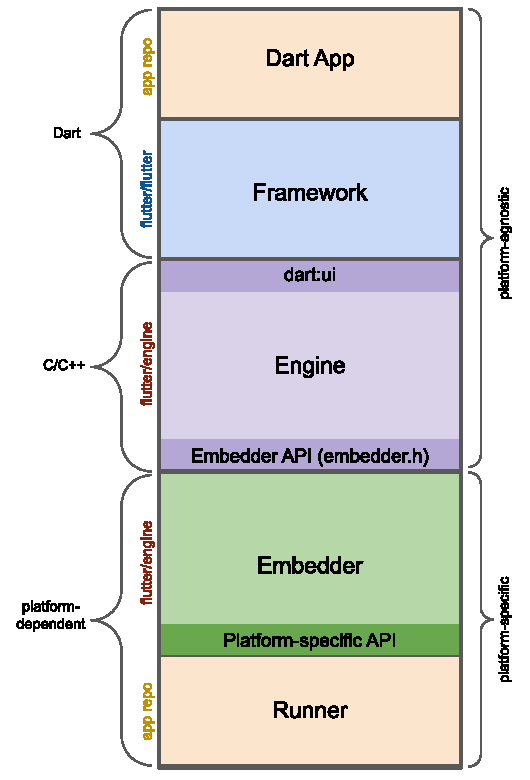
\includegraphics[scale=0.7]{flutter_architecture}
    \caption{Σχηματικό διάγραμμα της αρχιτεκτονικής δομής μίας εφαρμογής Flutter. Πηγή: \cite{flutter_architecture}}
\end{figure}

\begin{itemize}
    \item \textbf{Runner και Embedder}: Αποτελούν τη βάση της εφαρμογής και τον δίαυλο επικοινωνίας με το λογισμικό σύστημα.
    Είναι υπεύθυνα για την εκκίνηση της εφαρμογής, την ενημέρωσή της σχετικά με όλα τα system events, και τη δημιουργία του βάθρου πάνω στο οποίο ο engine θα εμφανίσει τα περιεχόμενα της εφαρμογής.
    Εφόσον τα δύο αυτά επίπεδα είναι άμεσα συνυφασμένα με το λογισμικό, ο σχετικός κώδικας είναι προσαρμοσμένος ειδικά για την εκάστοτε πλατφόρμα (πχ. χρησιμοποιείται Java/C++ για Android, και Objective-C για iOS)
    \item \textbf{Engine}: Αποτελεί τον πυρήνα μίας εφαρμογής Flutter. Συνιστάται από ένα runtime το οποίο εκτελεί τον κώδικα της εφαρμογής που είναι γραμμένος σε Dart, και χειρίζεται παράλληλα την εμφάνιση όλων των γραφικών στην οθόνη.
    Εφόσον επικοινωνεί με το λογισμικό διαμέσου του embedder, ο engine είναι ανεξάρτητος της πλατφόρμας (platform-agnostic)
    \item \textbf{Framework/Dart App}: Αποτελούν το υψηλού επιπέδου τμήμα της εφαρμογής.
    Το Flutter framework περιέχει όλα τα components με τα οποία ο προγραμματιστής θα συνθέσει την εφαρμογή, καθώς και εργαλεία για τον χειρισμό υπηρεσιών όπως τα animations και το gesture detection.
    Το τελευταίο επίπεδο είναι το μέρος της εφαρμογής που σχεδιάζεται εξ ολοκλήρου από τον developer, και περιέχει όλη τη λογική μαζί με το UI, όπως αυτά έχουν οριστεί από τον προγραμματιστή.
    Τόσο το Flutter framework όσο και ο κώδικας της εφαρμογής είναι γραμμένα στη γλώσσα Dart.
\end{itemize}

\section{Widgets}
Η βασική μονάδα όλων των στοιχείων του UI στο Flutter είναι το widget.
Ένα widget περιγράφει ένα μέρος του UI της εφαρμογής, όπως ένα κουμπί, κείμενο, ή εικονίδιο.

Πέρα από τα εμφανή λειτουργικά στοιχεία, στα widgets περιλαμβάνονται και στοιχεία που ελέγχουν την διάταξη/layout της εφαρμογής, όπως τα widget στοίχισης, padding, και δημιουργίας στηλών/γραμμών.
Η εφαρμογή έχει ως ρίζα ένα βασικό widget το οποίο αποτελεί το υπόβαθρο του συνόλου της διεπαφής, και όλα τα στοιχεία του UI δομούνται μέσα από την σύνθεση και την εμφώλευση απλότερων widget.
Ο κεντρικός αυτός ρόλος των widget δικαιολογεί το σλόγκαν που έχει υιοθετήσει το Flutter, \textit{``everything is a widget''}.

\bigskip

Το σύνολο των widget που απαρτίζουν μία εφαρμογη Flutter έχει τη δομή ενός δέντρου, με το κάθε widget να διαθέτει έναν γονιό (το widget μέσα στο οποίο είναι εμφωλευμένο) και ενδεχόμενα παιδιά (τα widget τα οποία περιέχει).

Στην πραγματικότητα το Flutter δεν ορίζει εσωτερικά το δέντρο των widget απευθείας, αλλά δομεί το λεγόμενο element tree του οποίου οι κόμβοι αντιστοιχούν στα widgets που όριζονται στον κώδικα, μαζί με όσα μεταβατικά widgets βρίσκονται ενδιάμεσά τους.
Επιπλέον, δεν ορίζεται μόνο ένα δένδρο, αλλά δύο· για λόγους απόδοσης, εκτός από το element tree ορίζεται και ένα render tree το οποίο περιέχει πληροφορίες για το rendering (δηλαδή τη σχεδίαση) των αντίστοιχων widget στην οθόνη.

Τα δέντρα αυτά αποτελούν το πιο σημαντικό μέρος του Flutter καθώς όλες οι διαδικασίες ενημέρωσης του UI στηρίζονται στην διάτρεξή τους και στην τροποποίηση των κόμβων τους.

\begin{quote}
    \nobreak
    \singlespacing
    \small
    ``Flutter is, at its core, a series of mechanisms for efficiently walking the modified parts of trees, converting trees of objects into lower-level trees of objects, and propagating changes across these trees.''

    \hfill{Flutter docs\cite{flutter_architecture}}
\end{quote}

\begin{figure}
    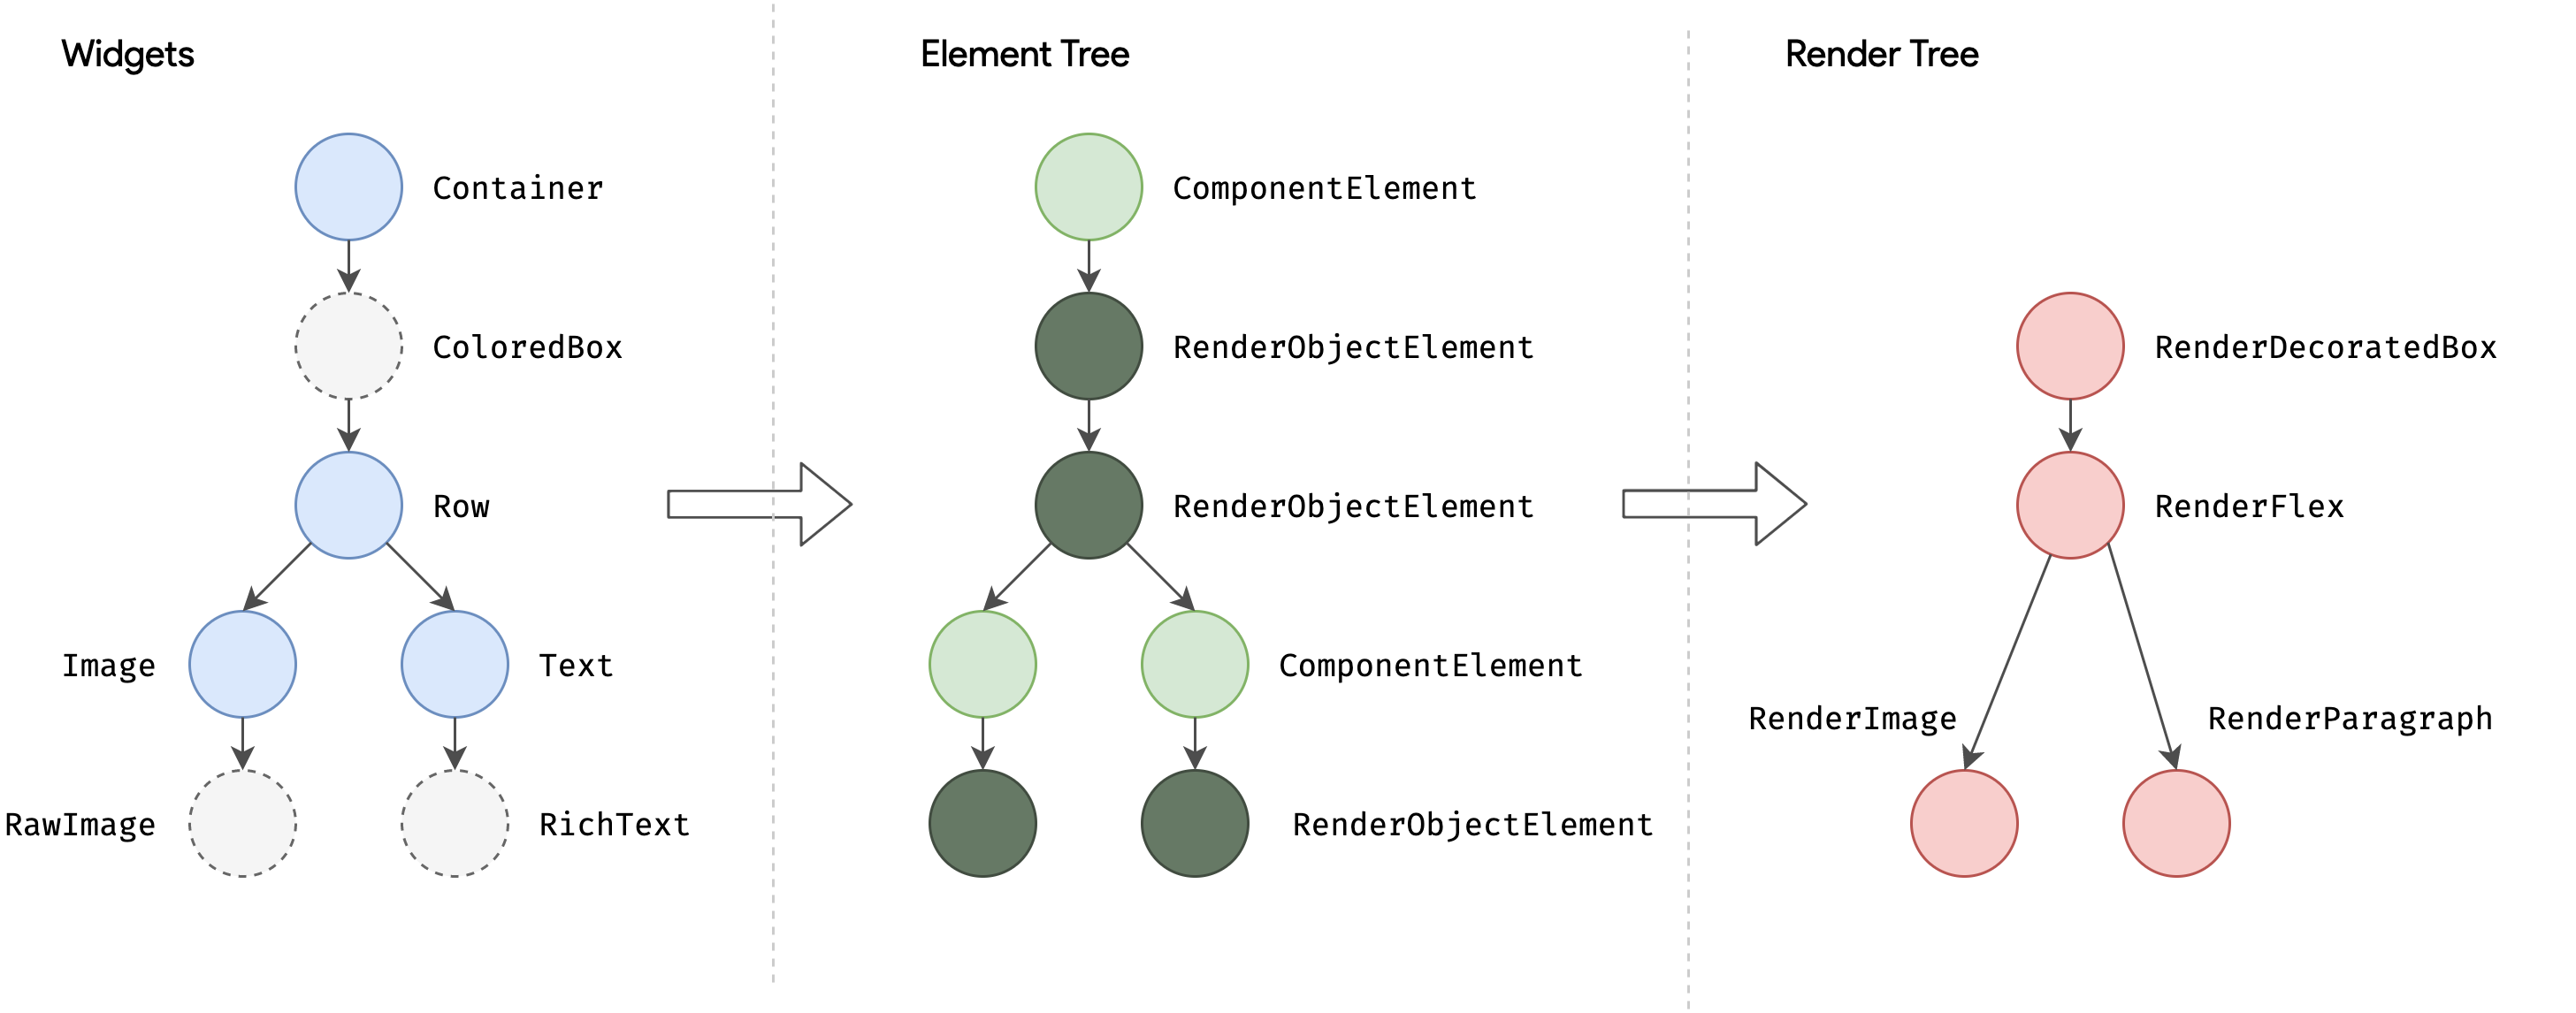
\includegraphics[width=\textwidth]{flutter_trees.png}
    \centering
    \caption{Δείγμα της ιεραρχίας των widgets με τη μορφή δέντρων. Πηγή: \cite{flutter_architecture}}
\end{figure}

\section{UI architecture}

Όλες οι εφαρμογές που διαθέτουν γραφικό περιβάλλον χρειάζονται έναν τρόπο να ανανεώνουν τα στοιχεία του UI τους σύμφωνα με τις δράσεις του χρήστη, και γενικότερα σύμφωνα με τις αλλαγές στην εσωτερική κατάσταση της εφαρμογής.

Ένας απλοϊκός τρόπος υλοποίησης του παραπάνω περιλαμβάνει την αρχική δημιουργία του UI, και έπειτα την συνεχή ανανέωση των χαρακτηριστικών των στοιχείων του μέσω του κώδικα.
Αυτή η μέθοδος γρήγορα γίνεται μη βιώσιμη για εφαρμογές που διαθέτουν κάποια στοιχειώδη πολυπλοκότητα, καθώς η μίξη κώδικα/λογικής και UI/εμφάνισης οδηγεί σε ανοργάνωτο κώδικα ο οποίος είναι επιρρεπής σε σφάλματα και είναι δύσκολα επεκτάσιμος.

\bigskip

Μία από τις πρώτες λύσεις στο πρόβλημα αυτό εμφανίστηκε υπό τη μορφή του μοτίβου \textit{Model-View-Controller (MVC design pattern)}.
Σύμφωνα με το MVC pattern, ο κώδικας της εφαρμογής που αφορά το UI χωρίζεται γενικά σε τρία μέρη, το model, το view και τον controller\cite{mvc_mdn}:
\begin{itemize}
    \item Το model αφορά το μέρος του κώδικα το οποίο περιγράφει τη δομή των δεδομένων που παρουσιάζονται στο UI, και αποτελεί την ``πηγή αλήθειας'' για τα δεδομένα αυτά. Είναι ουσιαστικά η εσωτερική κατάσταση της εφαρμογής, και έχει πλήρης άγνοια για την κατάσταση του UI.
    \item Το view έχει να κάνει αποκλειστικά με το μέρος του κώδικα που περιγράφει το UI της εφαρμογής, και είναι το κομμάτι με το οποίο αλληλεπιδρά άμεσα ο χρήστης. Εξαρτάται από τα δεδομένα που βρίσκονται στο αντίστοιχο model, και επομένως πρέπει να παρακολουθεί συνεχώς το model για αλλαγές ώστε να ενημερώνει την εμφάνισή του αναλόγως.
    \item Ο controller αποτελείται από κώδικα που λειτουργεί ως διαμεσολαβητής μεταξύ model και view. Δέχεται τα inputs του χρήστη από το view και ενημερώνει κατάλληλα το model για τις αλλαγές που επιφέρει η κάθε κίνηση του χρήστη στην κατάσταση της εφαρμογής, ενώ μπορεί ενδεχωμένως να ενημερώσει και άμεσα το view.
\end{itemize}
Με τον διαχωρισμό του κώδικα σε επιμέρους τμήματα, το καθένα με την δική του αρμοδιότητα, επιτυγχάνεται το λεγόμενο separation of concerns και συγκεκριμένα \textit{separation of content and presentation}\cite{mvc_fowler}: το UI αποζεύεται από την λογική του προγράμματος, γεγονός που οδηγεί σε πιο εύκολα κατανοητό και επεκτάσιμο κώδικα.
Το μοντέλο MVC είναι από τα παλαιότερα του είδους και εμφανίζει πολλαπλές παραλλαγές, οι οποίες είναι μέχρι και σήμερα σε εξαιρετικά ευρεία χρήση.

\bigskip

Το Flutter είναι ένα \textit{reactive framework}\footnote{Τα reactive frameworks βασίζονται στη φιλοσοφία της open-source βιβλιοθήκης \textit{React} που αναπτύσσεται από την εταιρία Meta (Facebook) από το 2013.} το οποίο επίσης προσπαθεί να ενσωματώσει το separation of concerns στο UI των εφαρμογών, υιοθετώντας όμως μία διαφορετική φιλοσοφία από το MVC.

Στο Flutter το UI της εφαρμογής περιγράφεται ορίζοντας τα widgets που το αποτελούν.
Τα widgets είναι immutable, και η ακριβής εμφάνισή τους είναι συνάρτηση της κατάστασης/state της εφαρμογής την στιγμή δημιουργίας τους, με την μέθοδο \texttt{build()} να είναι αρμόδια για τη δόμηση του κάθε widget δεδομένου του state. 
Επομένως, η αλλαγή της κατάστασης της εφαρμογής πρέπει να συνοδεύεται από την εκ νέου δημιουργία των widgets τα οποία πρέπει να αλλάξουν, δηλαδή από την κλήση της μεθόδου \texttt{build()}.
Ο ρόλος του Flutter είναι ουσιαστικά η στρατηγική ενημέρωση του widget tree (συγκεκριμένα του render tree) όποτε αυτή είναι απαραίτητη, με όσο το δυνατόν περισσότερο αποδοτικό τρόπο και χωρίς περιττές ανανεώσεις των widgets, έτσι ώστε να επιτυγχάνονται υψηλές επιδόσεις.

\section{State Management}
Έχοντας κάνει λόγο για την σημασία της κατάστασης/state στη λειτουργία της εφαρμογής, διακρίνουμε δύο ευρείες κατηγορίες του state εντός του πλαισίου του Flutter: ephemeral και application\cite{flutter_state}.

Η εφήμερη κατάσταση (αλλιώς local/UI state) είναι η κατάσταση ενός μεμονωμένου widget, οι οποία περιορίζεται εντός του widget αυτού και δεν αλληλεπιδρά με άλλα μέρη της εφαρμογής.
Η κατάσταση αυτή είναι συνήθως απλή, και αφορά κυρίως την εμφάνιση του widget και όχι κάποια σύνθετη δομή δεδομένων.
Η κλάση \texttt{StatefulWidget} αναπαριστά ένα widget που διαθέτει ephemeral state, και συνοδεύεται από την αντίστοιχη κλάση \texttt{State} η οποία περιέχει ακριβώς τα δεδομένα της κατάστασης του στοιχείου
Η μέθοδος \texttt{build()} ορίζεται εντός της κλάσης State, και περιγράφει τη δομή του widget συναρτήσει της κατάστασης της κλάσης.

Όταν η κατάσταση του widget αλλάζει έτσι ώστε να χρειάζεται η ανανέωση του UI, τότε το Flutter πρέπει να ειδοποιηθεί καταλλήλως ώστε να καλέσει τη μέθοδο build().
Αυτό ακριβώς επιτυγχάνεται μέσω της μεθόδου \texttt{setState()}, η οποία καλείται εντός του δεδομένου widget, σημειώνοντάς το ως ``dirty'' και σηματοδοτώντας στο Flutter την ανάγκη κλήσης της build() ώστε το UI να ανανεωθεί με τα νέα δεδομένα.

\bigskip

Το application (ή shared) state από την άλλη είναι η κατάσταση της εφαρμογής που δεν περιορίζεται σε ένα widget, αλλά την οποία μοιράζονται πολλαπλά διαφορετικά μέρη του UI.
Το γεγονός ότι το app state δεν ανήκει σε ένα μόνο widget παρουσιάζει το εξής πρόβλημα: πως μπορεί ένα widget να έχει πρόσβαση στο app state σε οποιοδήποτε μέρος του δέντρου και αν βρίσκεται, και πως μπορεί η πρόσβαση αυτή να γίνεται με τον πιο απλό, ασφαλή, αλλά και αποδοτικό τρόπο;

\bigskip

Η απάντηση σε αυτό το ερώτημα βασίζεται στην τακτική που ονομάζεται \textit{``lifting state up''}, την οποία μπορούμε να μεταφράσουμε ως ``αναγωγή κατάστασης''.
Μέσω της αναγωγής κατάστασης, η κατάσταση που μοιράζονται πολλαπλά στοιχεία μεταφέρεται σε έναν κόμβο που βρίσκεται ανώτερα στο δέντρο από τα στοιχεία αυτά.
Με άλλα λόγια, το shared state μεταφέρεται σε κόμβο που αποτελεί \textit{κοινό πρόγωνο} των στοιχείων στο δέντρο.

Το shared state, ως parent πια των εμπλεκόμενων widgets, μπορεί να ειδοποιεί όλα τα widget-παιδιά του για αλλαγές στην κατάσταση, ενώ το κάθε widget-παιδί λαμβάνει πρόσβαση στο shared state αφού το αναζητήσει διατρέχοντας τους απογόνους του του δέντρου.

Οι μηχανισμοί για τη παραπάνω λειτουργία προσφέρονται από την βιβλιοθήκη \texttt{provider}\cite{flutter_provider}, η οποία χρησιμοποιείται κατά κόρον και από την ομάδα του Flutter.
Η βιβλιοθήκη παρέχει τους λεγόμενους \texttt{Provider} οι οποίοι απλά περικλείουν την κλάση που αποτελεί το shared state, κάνοντάς τήν εύκολα διαθέσιμη στα υπόλοιπα μέρη της εφαρμογής.
Ωστόσο, σε συνδυασμό με την κλάση \texttt{ChangeNotifier} η οποία είναι μέρος του Flutter framework, ένας Provider μπορεί επιπροσθέτως να ειδοποιεί τα widget που έχουν πρόσβαση στο shared state κάθε φορά που η κατάσταση μεταβάλλεται, πυροδοτώντας την ανανέωσή τους.

Τα στοιχεία που επιθυμούν να παρακολουθούν έναν Provider περικλείονται από ένα widget \texttt{Consumer} το οποίο αναλαμβάνει την ακρόαση του state που παρέχει ο συγκεκριμένος Provider και χειρίζεται αυτόματα το rebuild του εσωκλειόμενου widget.
Με αυτόν τον τρόπο έχουμε πλήρως αυτόματο συγχρονισμό του shared state και ενημέρωση του UI από οποιοδήποτε μέρος της εφαρμογής σε οποιοδήποτε άλλο, υλοποιώντας πλήρως τη φιλοσοφία του reactive programming.

\begin{figure}
    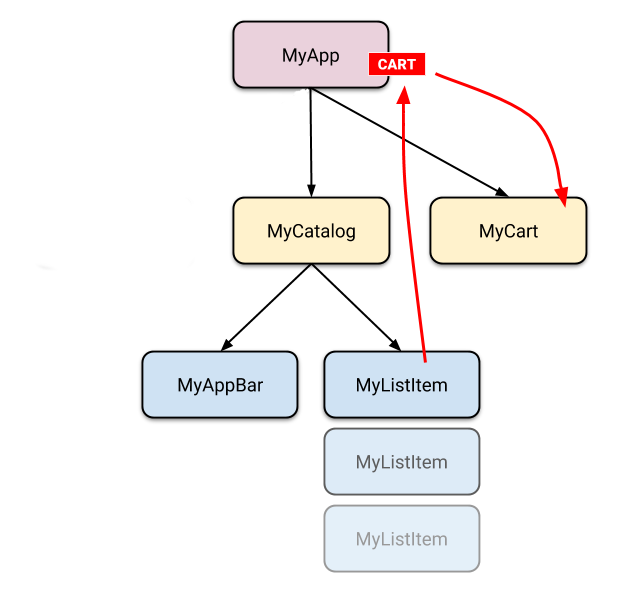
\includegraphics[width=\textwidth]{flutter_provider_example.png}
    \centering
    \caption{Παράδειγμα αναγωγής κατάστασης. Η δεδομένη εφαρμογή περιέχει ένα μία λίστα από widgets \texttt{MyListItem} που αποτελούν τα προϊόντα ενός e-shop, και ένα widget \texttt{MyCart} που εμφανίζει τα προϊόντα που έχουν προστεθεί στο καλάθι. Τόσο τα MyListItem όσο και το MyCart πρέπει να έχουν πρόσβαση σε μία κλάση που αναπαριστά το καλάθι του χρήση, αφού για παράδειγμα όταν ένα MyListItem πατηθεί το αντίστοιχο προϊόν πρέπει να προστίθεται στο καλάθι και ταυτόχρονα να εμφανίζεται στο MyCart. Έτσι δημιουργείται ένας provider \texttt{Cart} που περιέχει την κατάσταση του καλαθιού, και τοποθετείται στον κοινό πρόγονο του MyListItem και του MyCart δηλαδή στο \texttt{MyApp}. Η προσθήκη ενός προϊόντος από το MyListItem προσπελάζει τον provider Cart, ο οποίος ειδοποιεί αμέσως το MyCart για την αλλαγή. Πηγή: \cite{flutter_state}}
\end{figure}

\end{document}